\section{Proposed System}
\vspace{1em}  
The proposed system aims to enhance the existing process of monitoring temperature in a drying and firing tunnel by introducing automation through microprocessor-based instrumentation. For this purpose we require the following components.
\vspace{1em}
\begin{itemize}
    \item Microprocessor
    \item Programmable Peripherial Interface (PPI) 
    \item Multiplexer
    \item Analog To Digital COnverter (ADC)
    \item Liquid Level sensors
    \item Counter
\end{itemize}
\vspace{2em}
\begin{figure}[h]
    \centering
    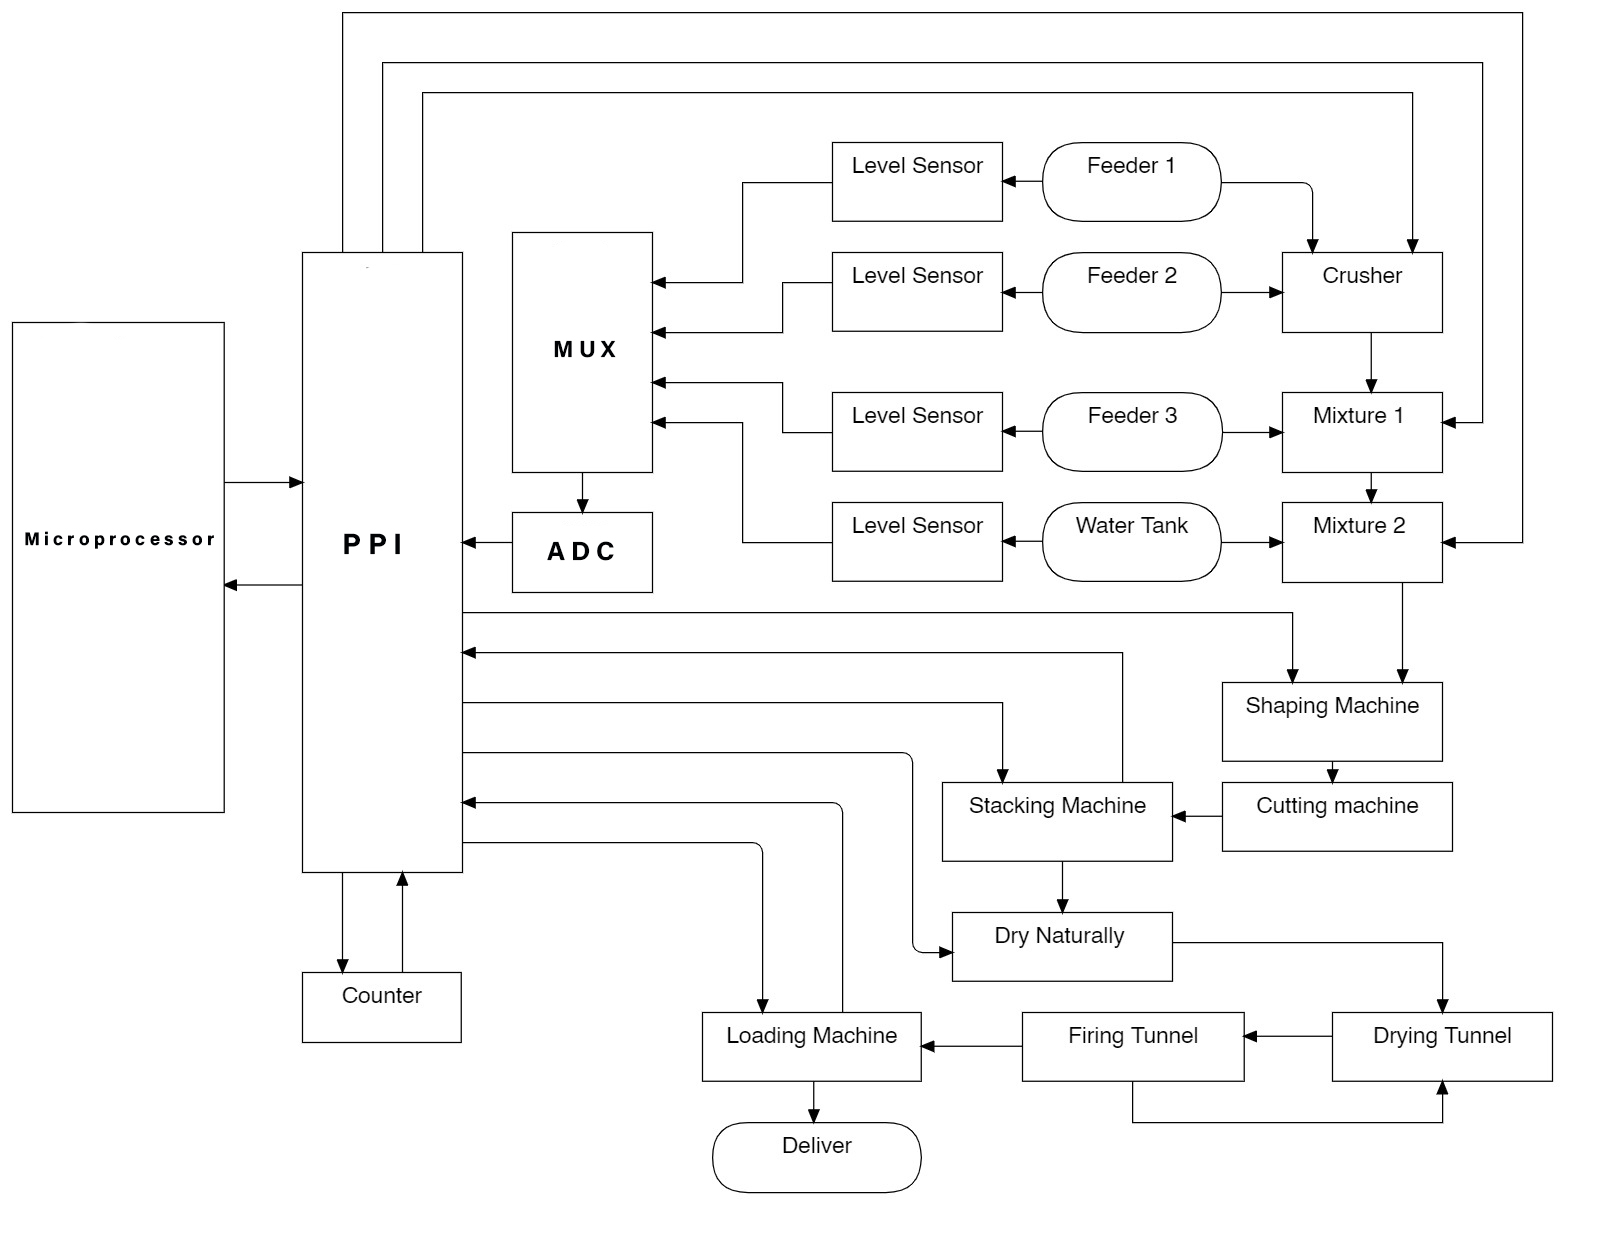
\includegraphics[width=1\textwidth]{img/fc.jpg}
    \caption{Block diagram for proposed system}
\end{figure}
\vspace{5em}
The block diagram provided visually represents the architecture of the proposed system. The system takes input from level sensors placed on different feeders and a water tank to monitor material availability. Once enough material for a batch is detected, the microprocessor initiates control signals to activate different elements for starting their operations. If there is insufficient material for the next batch, the system can notify in advance to refill the feeder. Similarly, if there's not enough material for the current batch, the microprocessor sends signals to halt ongoing processes.

When a batch of bricks is stacked, the stacking machine sends a signal to the microprocessor, which then instructs the counter to start counting. After 12 hours (or a specified time interval), the counter informs the microprocessor, which subsequently sends signals to the motors to transfer the batch from the natural drying zone to the drying tunnel.

After the batch exits the firing tunnel, a loading machine loads the batch onto a delivery truck when the truck becomes available. The microprocessor plays a crucial role in coordinating this process. It receives signals indicating when the batch is ready for delivery and when the delivery truck arrives. Upon truck arrival, the microprocessor sends a signal to the loading machine, directing it to load the batch onto the truck for delivery.

This proposed system aims to streamline the brick manufacturing process by automating various stages, optimizing material usage, and improving overall operational efficiency. By utilizing microprocessor-based control and monitoring, the system reduces manual intervention and enhances the accuracy of various processes involved in brick production and delivery.